%!TEX root = ../../../main.tex

\section[VCSELs]{Coupling \sivs to \Vcsels} \label{sec::coupling_vcsel}

	For metrology, the photon flux rate has to be high enough to be measured by a low optical flux detector \cite{Vaigu2017}.
	\\
	The red AlGaInP-based oxide-confined \vcsels (VCSEL) are compact and perfect candidates for excitation of \sivs in a hybrid integrated single photon source: 
	They exhibit wavelengths around \SI{650}{nm} at \cw emission.
	\sivs exhibit intensity maxima at an excitation at \SI{670}{nm} and \SI{690}{nm} \cite{}.\todo{diagram einfuegen} 
	In addition, VCSELs exhibit circular beam profile, have low divergence angle and emit linearly polarized light.

	\subsection{\Vcsel Structure}\label{subsec::vcsel_structure}

	% Vertical-cavity surface-emitting lasers are attractive candidates for emerging technologies such as high-density optical storage systems, high-definition laser printing and optical communication systems using polymer optical fibers (POF). The red AlGaInP-based oxide-confined vertical-cavity surface-emitting lasers (VCSEL) target one absorption minimum of the polymer optical fibers (POF) at around 650 nm. In addition, VCSELs are compact, exhibit circular beam profile and have low divergence angle, in contrast to edge-emitting laser, for an easy coupling of light into the fiber. Furthermore, they offer high-speed modulation capability (several GHz) [1] which is required for optical data communication.
	% \\
	% The VCSEL structure (Fig. 2) consists of an laser active region embedded in between two distributed Bragg reflectors (DBR). For maximum modal gain the current and the optical mode need to be confined in the transverse direction for serving as a spatial filter. This is achieved with an implemented oxide aperture, with diameter DA, directly above the active region in a field node of the standing wave field to minimize scattering losses. Our devices possess optical output power up to 3 mW with low threshold current (1 mA) at 660 nm. For practical application a stable single transverse mode especially the fundamental mode and a stable polarization of the emission is desirable owing to higher coupling-efficiency into optical fibers.
	% \\
	% II. EXPERIMENTAL PROCEDURE The investigated VCSEL structures were grown by metalorganic vapor-phase epitaxy (MOVPE) in an AIX-200 hori- zontal reactor setup with in situ growth control using stan- dard sources at low pressure of 100 mbar and a tempera- ture of 750 ◦C on (100) n+-GaAs substrate misoriented 6 ◦ towards [111]A. The bottom n-type DBR is made of 50 pairs of AlAs/Al0.5Ga0.5As. The p-type DBR consists of 36 Al0.95Ga0.05As/Al0.5Ga0.5As mirror pairs. Four compres- sively strained GaInP quantum wells (QW) built up the active region. To realize an oxide aperture, the advantage of high oxidation selectivity of the AlxGa1−xAs material system is used. We use an Al-content of x = 0.98 for this oxidation layer. Active diameters DA from 3 µm to 20 µm were obtained on one sample because of the flow profile of the nitric water vapor in the oxidation chamber. To investigate the transverse beam profile depending on different parameters we built up a vertical measurement setup. The beam profile is mapped with a lens system of 3 lenses and captured with a CMOS-camera. The vertical setup provides the advantage of on-wafer-testing.

	The VCSEL structure (\autoref{fig::vcsel_sketch}) consists of an active region between two distributed Bragg reflectors (DBR). 
	The bottom n-type DBR is made of 50 pairs of AlAs/Al\textsubscript{0.5}Ga\textsubscript{0.5}As, the p-type DBR consists of 36 Al\textsubscript{0.95}Ga\textsubscript{0.05}As/Al\textsubscript{0.5}Ga\textsubscript{0.5}As mirror pairs \cite{Weidenfeld2012}. 
	The active region consists of four GaInP quantum wells (QW). 
	An oxide aperture in a field node of the standing wave serves as a spatial filter for maximum modal gain by confining the current and the optical mode.
	The active diameter which is defined by the oxide aperture amounts to \SI{5.8}{\micro\meter}.
	As this region is the area where the laser emission exits the VCSEL, the \nds have to be put within this area.
	The used VCSEL exhibits an optical output power up to \SI{1}{\milli\watt} with low threshold current of up to \SI{3}{\milli\ampere}\todo{ist das up to} at about \SI{655}{nm}\todo{nachdenken, wie formulierung richtig ist}. 

	\begin{figure}[tp]
		\begin{subfigure}[t]{ 0.49\linewidth}
			\centering
			\testbox{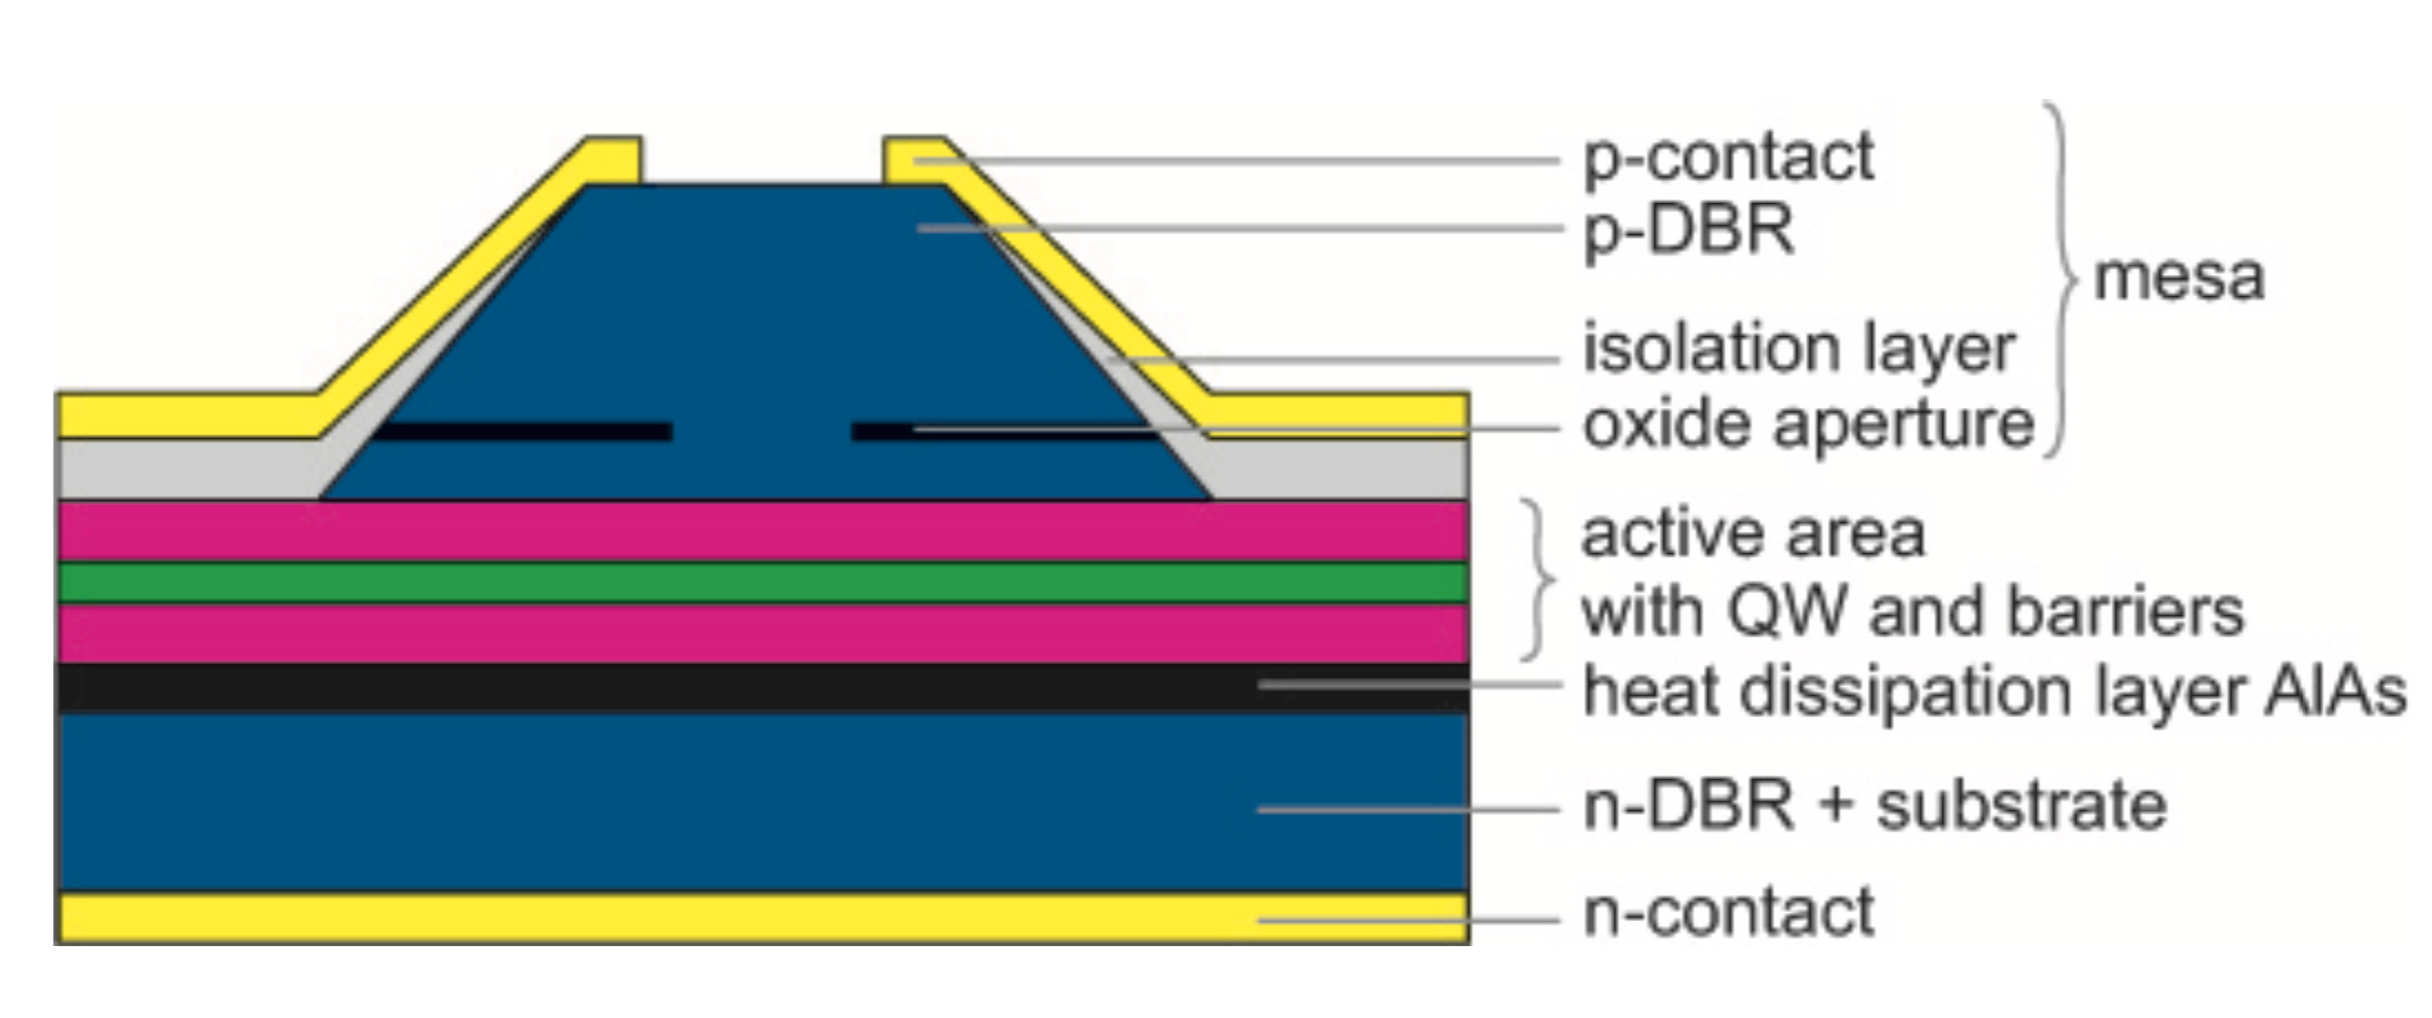
\includegraphics[trim = 0 0 0 0,  clip= true, width = \textwidth]{./pics/vcsel_sketch.png}}
			\caption{}
			\label{subfig::vcsel_sketch}
		\end{subfigure}
		\hfill
		\begin{subfigure}[t]{ 0.49\linewidth}
			\centering
			\testbox{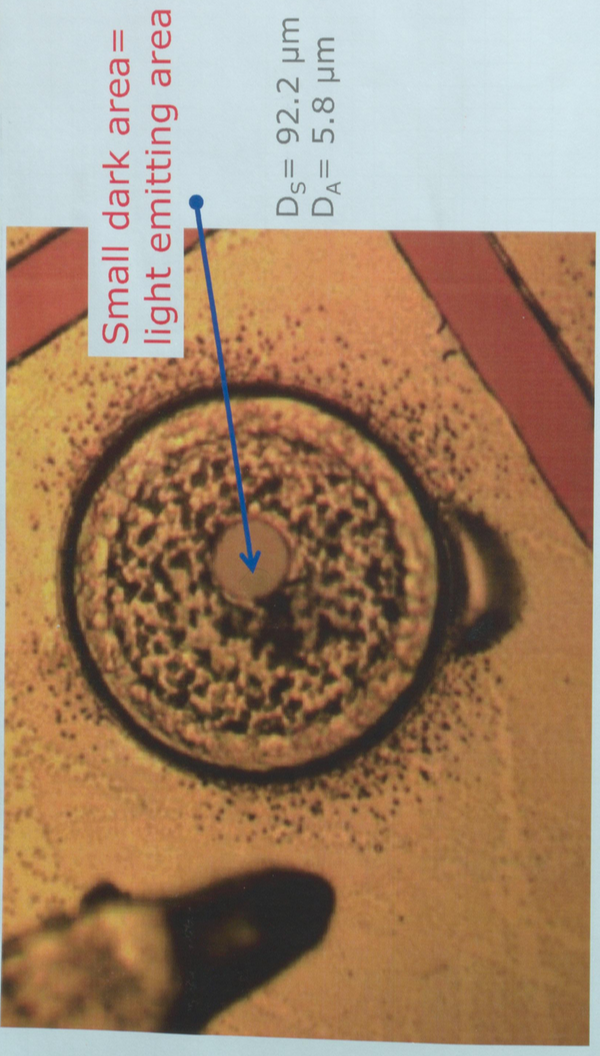
\includegraphics[trim = 0 0 0 0,  clip= true, width = \textwidth]{./pics/vcsel_output_area.png}}
			\caption{}
			\label{subfig::vcsel_output_area}
		\end{subfigure}
		\caption{(a) Sketch of the VCSEL showing the different layers. \todo[inline]{ask how to cite}(b) Image of the VCSEL. The circle with the black dots is the hole in the p-contact (diameter D\textsubscript{S}, the smaller darker area in the middle is the laser output area (diameter D\textsubscript{A})}
		\label{fig::<fig>}
	\end{figure}

	\begin{figure}[tp]
		\begin{subfigure}[t]{ 0.49\linewidth}
			\centering
			\testbox{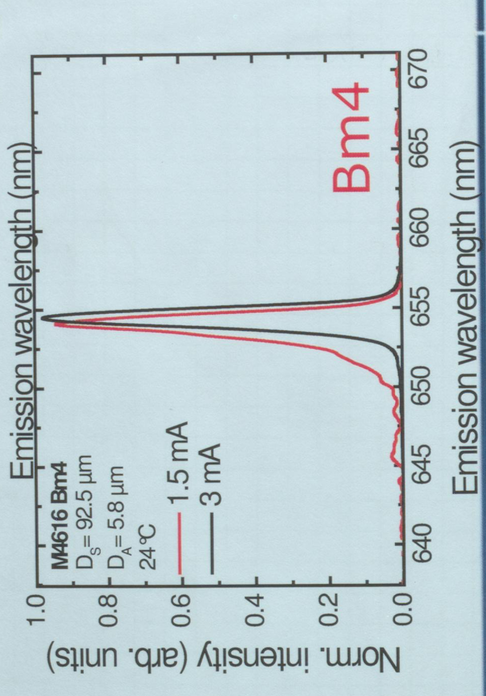
\includegraphics[trim = 0 0 0 0,  clip= true, width = \textwidth]{./pics/vcsel_output_wavelength.png}}
			\caption{}
			\label{subfig::vcsel_output_wavelength}
		\end{subfigure}
		\hfill
		\begin{subfigure}[t]{ 0.49\linewidth}
			\centering
			\testbox{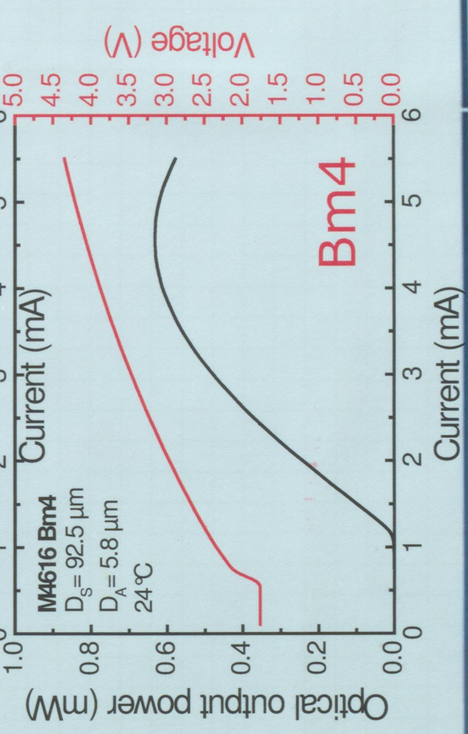
\includegraphics[trim = 0 0 0 0,  clip= true, width = \textwidth]{./pics/vcsel_output_power.png}}
			\caption{}
			\label{subfig::vcsel_output_power}
		\end{subfigure}
		\caption{(a) Emission spectrum of the used VCSEL at two different currents. (b) Optical output power and voltage of the same VCSEL in dependence of input current. \cite{}}
	\end{figure}

	\begin{figure}[tp]
		\begin{subfigure}[t]{ 0.49\linewidth}
			\centering
			\testbox{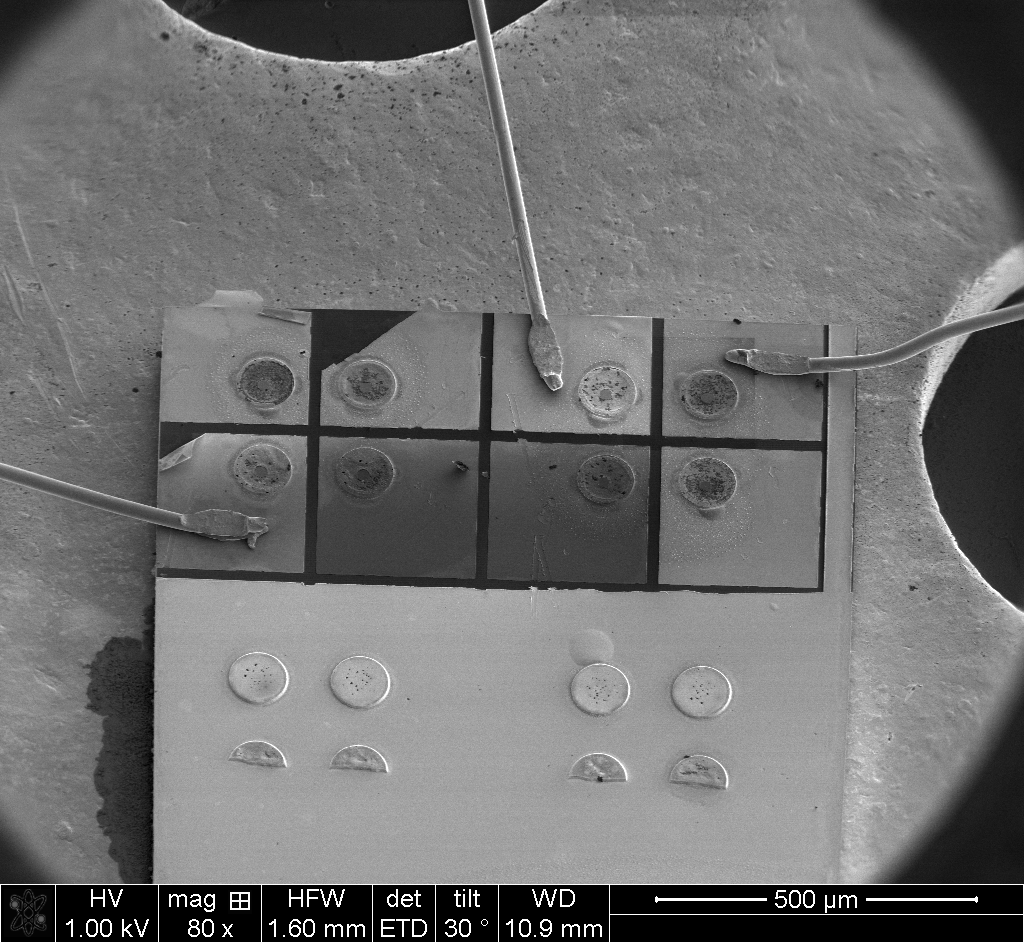
\includegraphics[trim = 0 0 0 0,  clip= true, width = \textwidth]{./pics/M05-13_PP_194_140926_13.png}}
			\caption{}
			\label{subfig::vcsel_sem_big_overview}
		\end{subfigure}
		\hfill
		\begin{subfigure}[t]{ 0.49\linewidth}
			\centering
			\testbox{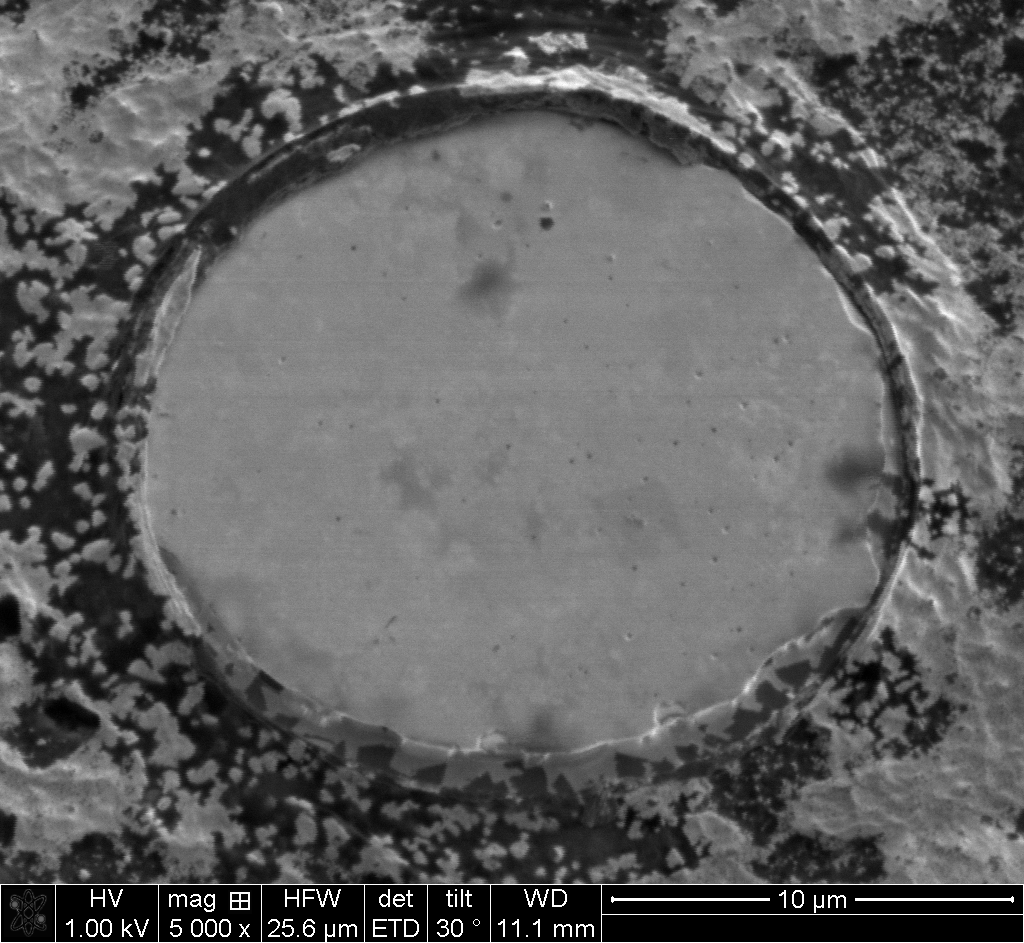
\includegraphics[trim = 0 0 0 0,  clip= true, width = \textwidth]{./pics/M05-13_PP_194_140926_14.png}}
{}			\caption{}
			\label{subfig::vcsel_sem_detail}
		\end{subfigure}
		\caption{(a) SEM image of an array of VCSELs. The three wires are the anodes, which are connected to the top layer (p-contact) of the VCSEL. Therefore, three of the VCSEL structures can be operated. (b) Detail SEM image of the top of the exploited VCSEL Bm4. The circular middle part is the hole in the p-contact through which the top DBR is visible. The active diameter is smaller than that and not visible in the SEM.}
	\end{figure}

	\subsection{\siv in a \Vcsel}

	% additional methods
	As diamond material we used CVD grown \nds.
	They had been grown on an \ir coated \si wafer (see \autoref{sec::cvd}).
	These \nds exhibit a nominal size of \SI{200}{nm}.
	% preselection, 
	First, we selected a \nd which exhibited one dominant line at \SI{746.0}{nm} with a \lw of \SI{1.9}{nm}\todo{was it single?}.
	% position
	Consecutively, its position on the substrate was determined using a white light laser scan as described in \autoref{subsec::position}.
	% transfer
	It was then transferred to the VCSEL Bm4 described in \autoref{subsec::vcsel_structure}.
	\\
	% Spectroscopic measurements
	After a successful transfer of the pre-selected \nd onto the active area of VCSEL Bm4, the VCSEL was put in the confocal setup.
	Using the laser from the confocal setup we checked if the \pp process caused any modification of the spectroscopic properties of the \siv such as a decrease of countrate or a modification of the \fl spectrum.
	For this, the VCSEL itself was not operated itself.
	First, the VCSEL surface was scanned \autoref{subfig::vcsel_confocal_laser_excitation_with_diamond}.
	.
	A bright dot exhibiting a countrate of a few thousand counts per second is visible where the \nd containing an SiV was put.
	A comparative scan of a VCSEL without \nd only exhibits a background countrate, as expected (\autoref{subfig::confocal_laser_excitation_without_diamond}).
	\\
	The spectrum of the \siv in the transferred \nd was investigated before and after the \pp process.
	The original spectrum before \nd transfer exhibits a sharp line at \SI{746.0}{nm}.
	After the \pp process, this line is still there, albeit with a low intensity.
	Another line at \SI{700}{nm} \todo{check number} which was a minor feature in the spectrum before \pp, is a sharp line after the process. 
	The explanation is, that 



	\begin{figure}[tp]
		\begin{subfigure}[t]{ 0.49\linewidth}
			\centering
			\testbox{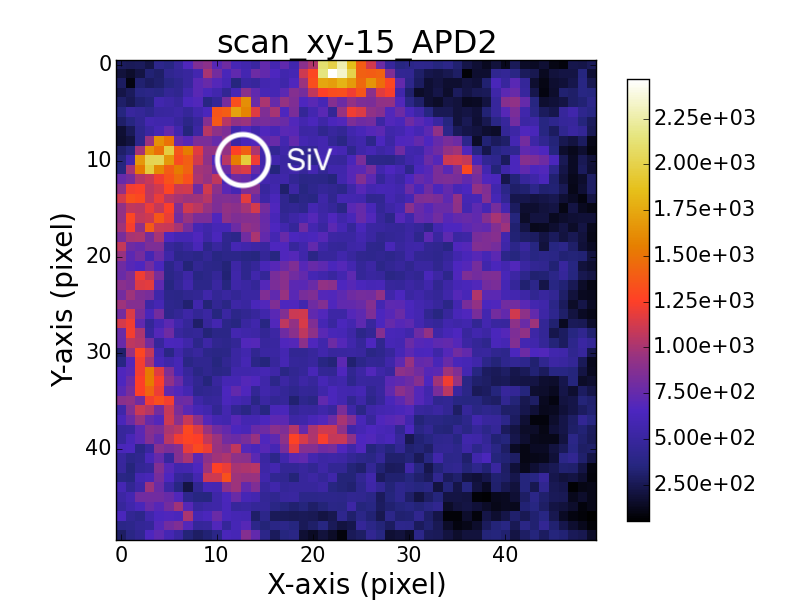
\includegraphics[trim = 0 0 0 0,  clip= true, width = \textwidth]{./pics/scan_xy-15_APD2_circle.png}}
			\caption{}
			\label{subfig::vcsel_confocal_laser_excitation_with_diamond}
		\end{subfigure}
		\hfill
		\begin{subfigure}[t]{ 0.49\linewidth}
			\centering
			\testbox{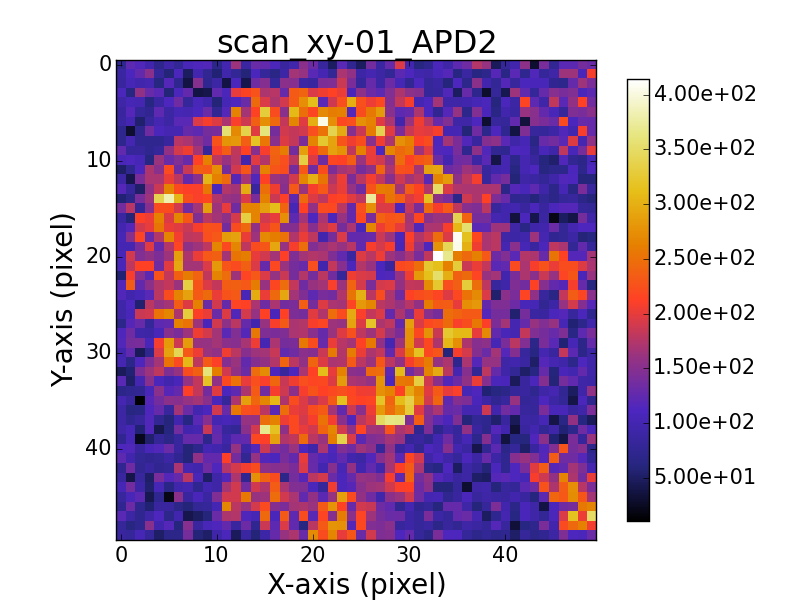
\includegraphics[trim = 0 0 0 0,  clip= true, width = \textwidth]{./pics/scan_xy-01_APD2.png}}
			\caption{confocal laser excitation without diamond}
			\label{subfig::confocal_laser_excitation_without_diamond}
		\end{subfigure}
		\caption{(a) Scan of the VCSEL Bm4 with coupled \nd under excitation with the laser from the confocal setup. The big visible ring is the edge of the cirular hole in the p-contact.The bright spot in the upper left corner corresponds to the transferred \nd containing an \siv. (b) Scan of the VCSEL Bm2 without \nd under excitation with the laser from the confocal setup. The cirular hole in the p-contact exhibits a constant countrate.}
	\end{figure}

	\begin{figure}[tp]
		\begin{subfigure}[t]{ 0.49\linewidth}
			\centering
			\testbox{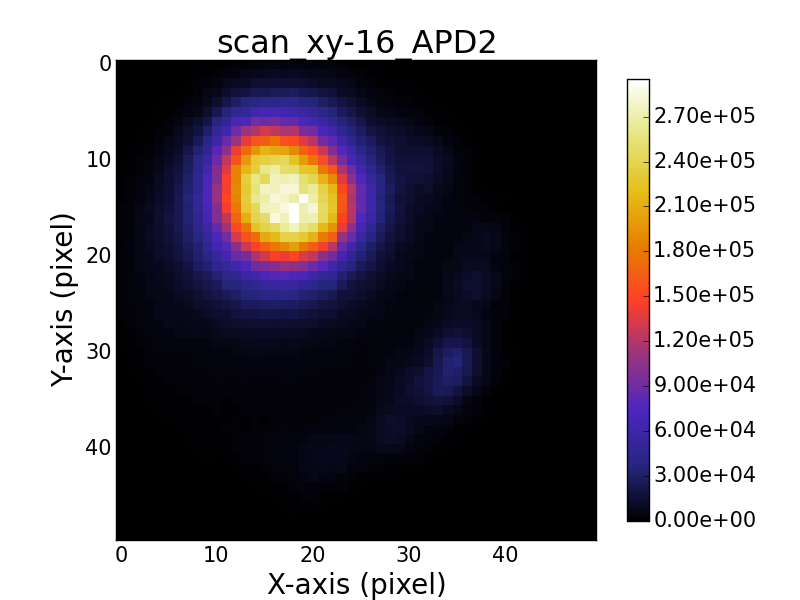
\includegraphics[trim = 0 0 0 0,  clip= true, width = \textwidth]{./pics/scan_xy-16_APD2.png}}
			\caption{vcsel excitation with diamond}
			\label{subfig::vcsel_excitation_with_diamond}
		\end{subfigure}
		\hfill
		\begin{subfigure}[t]{ 0.49\linewidth}
			\centering
			\testbox{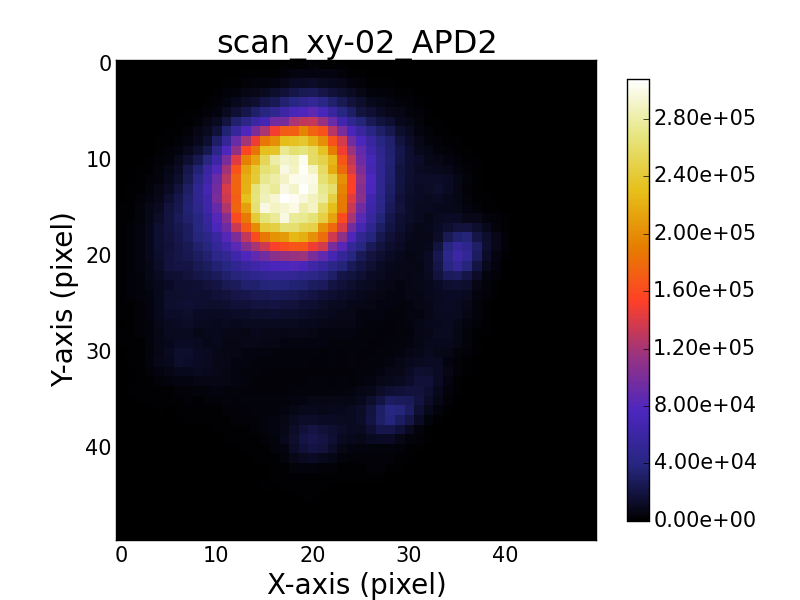
\includegraphics[trim = 0 0 0 0,  clip= true, width = \textwidth]{./pics/scan_xy-02_APD2.png}}
			\caption{vcsel excitation without diamond}
			\label{subfig::vcsel_excitation_without_diamond}
		\end{subfigure}
		\caption{<caption>}
	\end{figure}

	\begin{figure}[tp]
		\begin{subfigure}[t]{ 0.49\linewidth}
			\centering
			\testbox{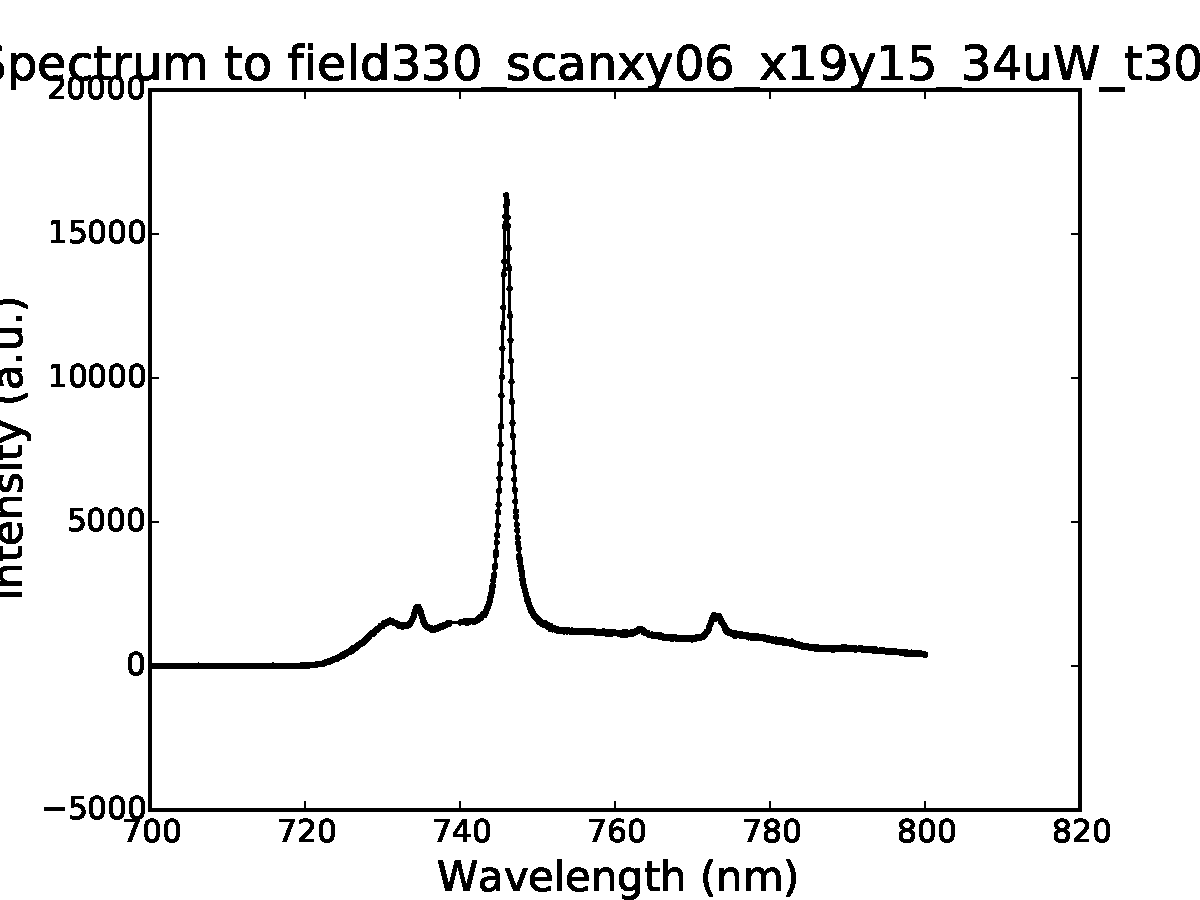
\includegraphics[trim = 0 0 0 0,  clip= true, width = \textwidth]{./pics/field330_scanxy06_x19y15_34uW_t30_2.pdf}}
			\caption{<caption>}
			\label{subfig::spectrum_diamond_for_vcsel_before_pp}
		\end{subfigure}
		\hfill
		\begin{subfigure}[t]{ 0.49\linewidth}
			\centering
			\testbox{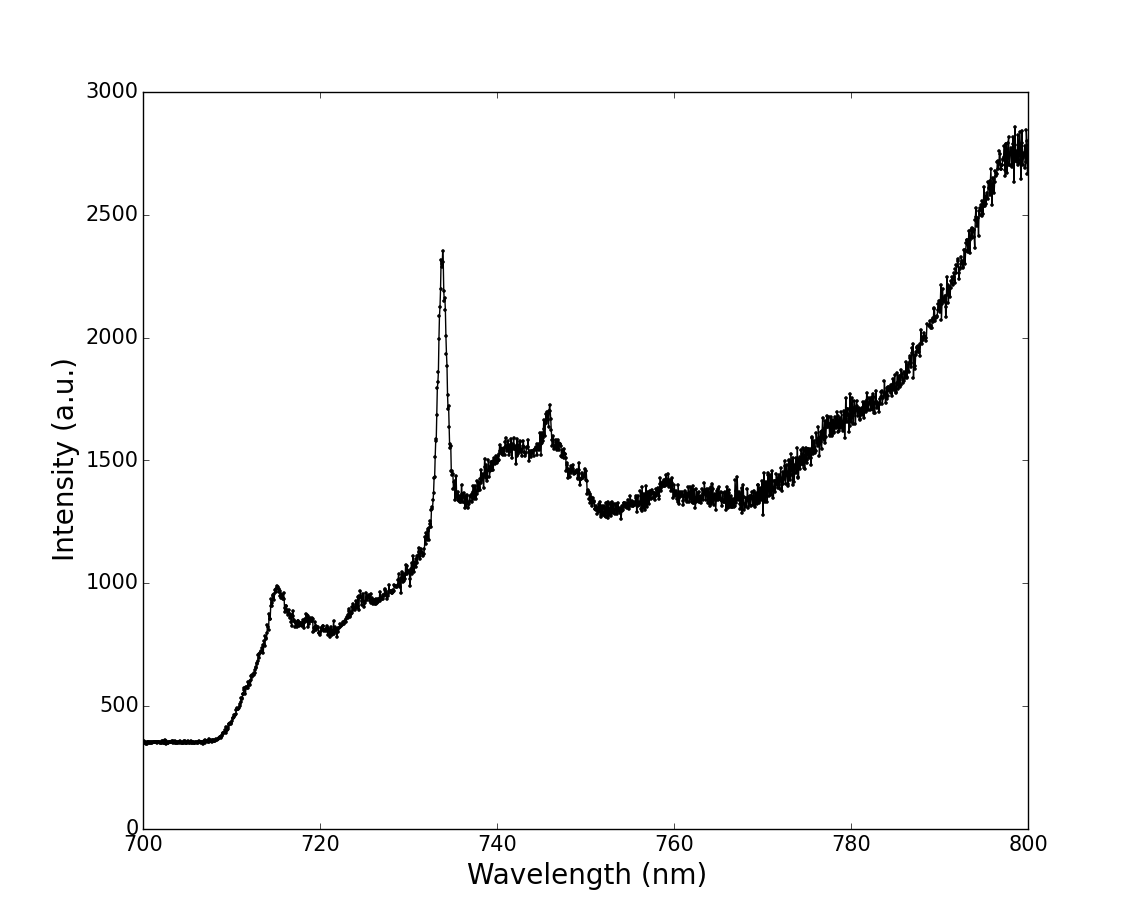
\includegraphics[trim = 0 0 0 0,  clip= true, width = \textwidth]{./pics/spe_scan_xy-25_300uW_t60_700-800nm.png}}
			\caption{<caption>}
			\label{subfig::spectrum_vcsel_confocal_excitation_with_diamond}
		\end{subfigure}
		\caption{<caption>}
		\label{fig::<fig>}
	\end{figure}

	% \begin{figure}[tp]
	% 	\begin{subfigure}[t]{ 0.49\linewidth}
	% 		\centering
	% 		\testbox{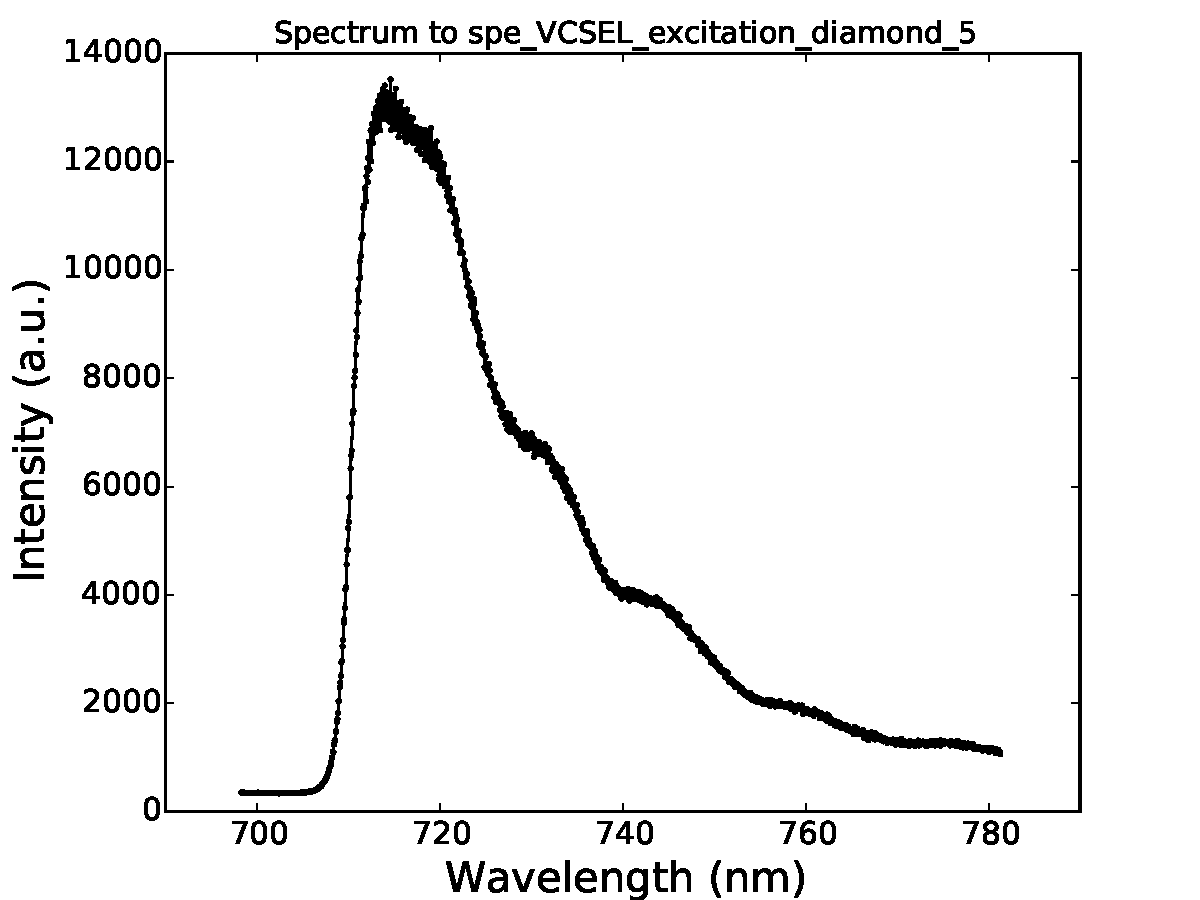
\includegraphics[trim = 0 0 0 0,  clip= true, width = \textwidth]{./pics/spe_VCSEL_excitation_diamond_5.pdf}}
	% 		\caption{spectrum vcsel excitation with diamond}
	% 		\label{subfig::spectrum_vcsel_excitation_with_diamond}
	% 	\end{subfigure}
	% 	\hfill
	% 	\begin{subfigure}[t]{ 0.49\linewidth}
	% 		\centering
	% 		\testbox{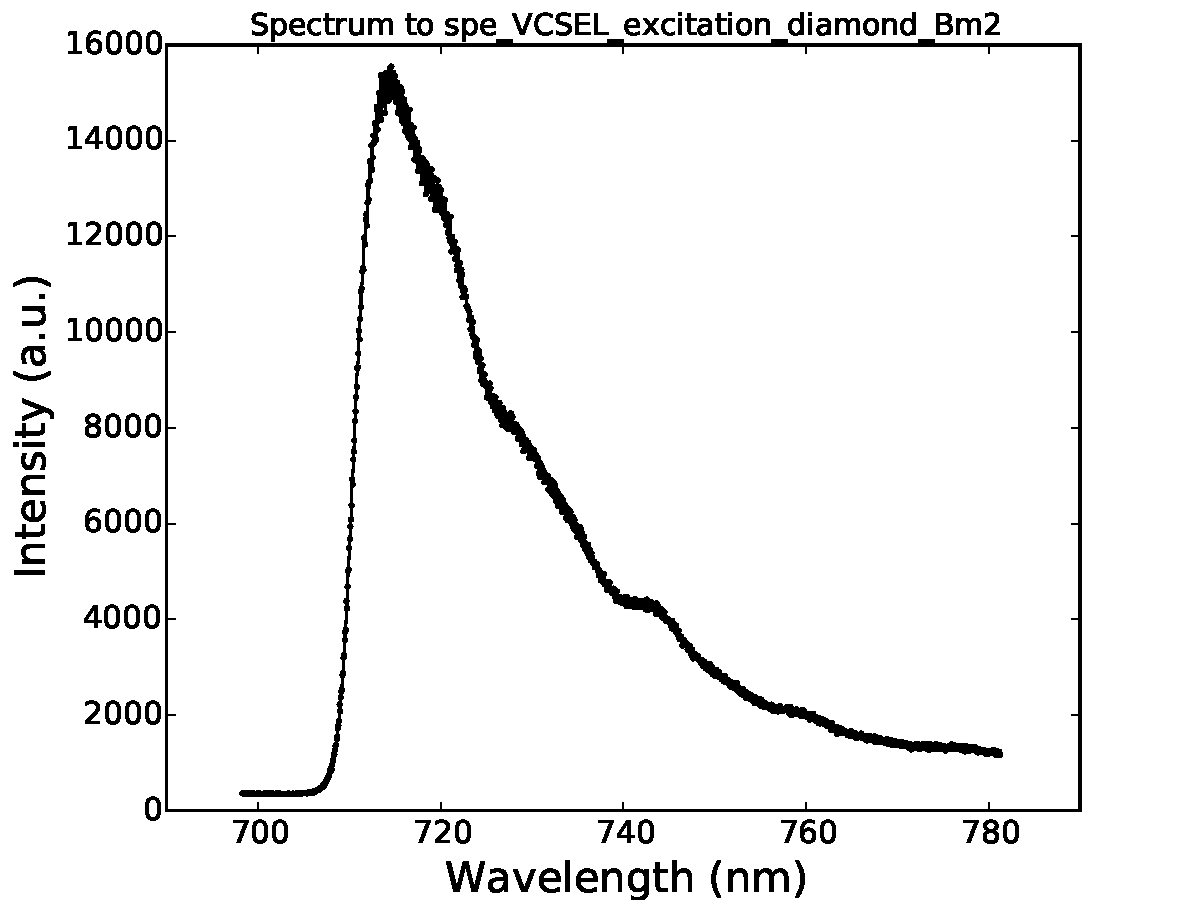
\includegraphics[trim = 0 0 0 0,  clip= true, width = \textwidth]{./pics/spe_VCSEL_excitation_diamond_Bm2.pdf}}
	% 		\caption{spectrum vcsel excitation without diamond}
	% 		\label{subfig::spectrum_vcsel_excitation_without_diamond}
	% 	\end{subfigure}
	% 	\caption{<caption>}
	% 	\label{fig::<fig>}
	% \end{figure}

	\begin{figure}[tp]
		\centering
		\testbox{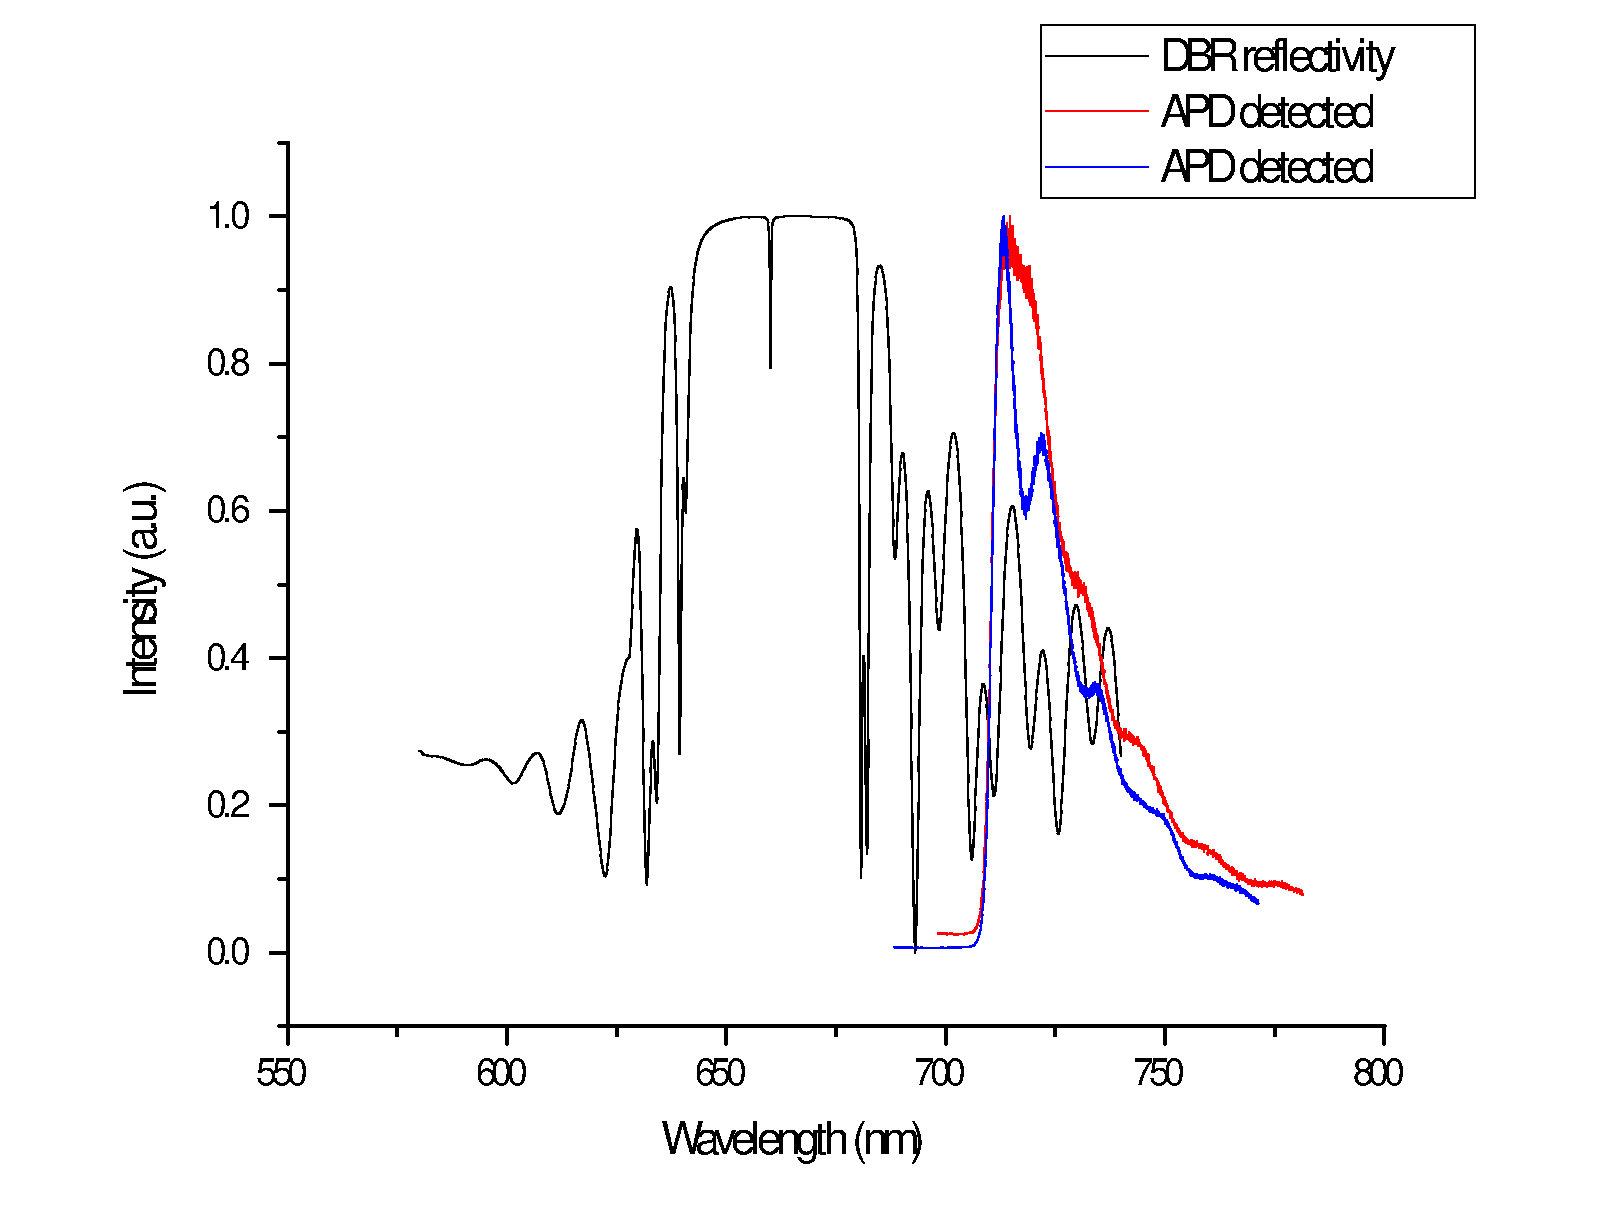
\includegraphics[trim = 0 0 0 0,  clip= true, width = 0.3\textwidth]{./pics/dbr_VCSEL.pdf}}
		\caption{Reflectivity of the DBR of the VCSEL, and spectra of the VCSEL measured in the confocal setup.}
		\label{fig::dbr_vcsel}
	\end{figure}